\chapter{Diagramas y Gráficos Detallados}
\label{chap:diagramas_detallados}

\lettrine{E}{n} este apéndice se incluyen los diagramas detallados y gráficos extensos que complementan el desarrollo del proyecto.

\section{Diagrama de flujo completo del sistema de tracking}

\begin{figure}[h!]
	\centering
	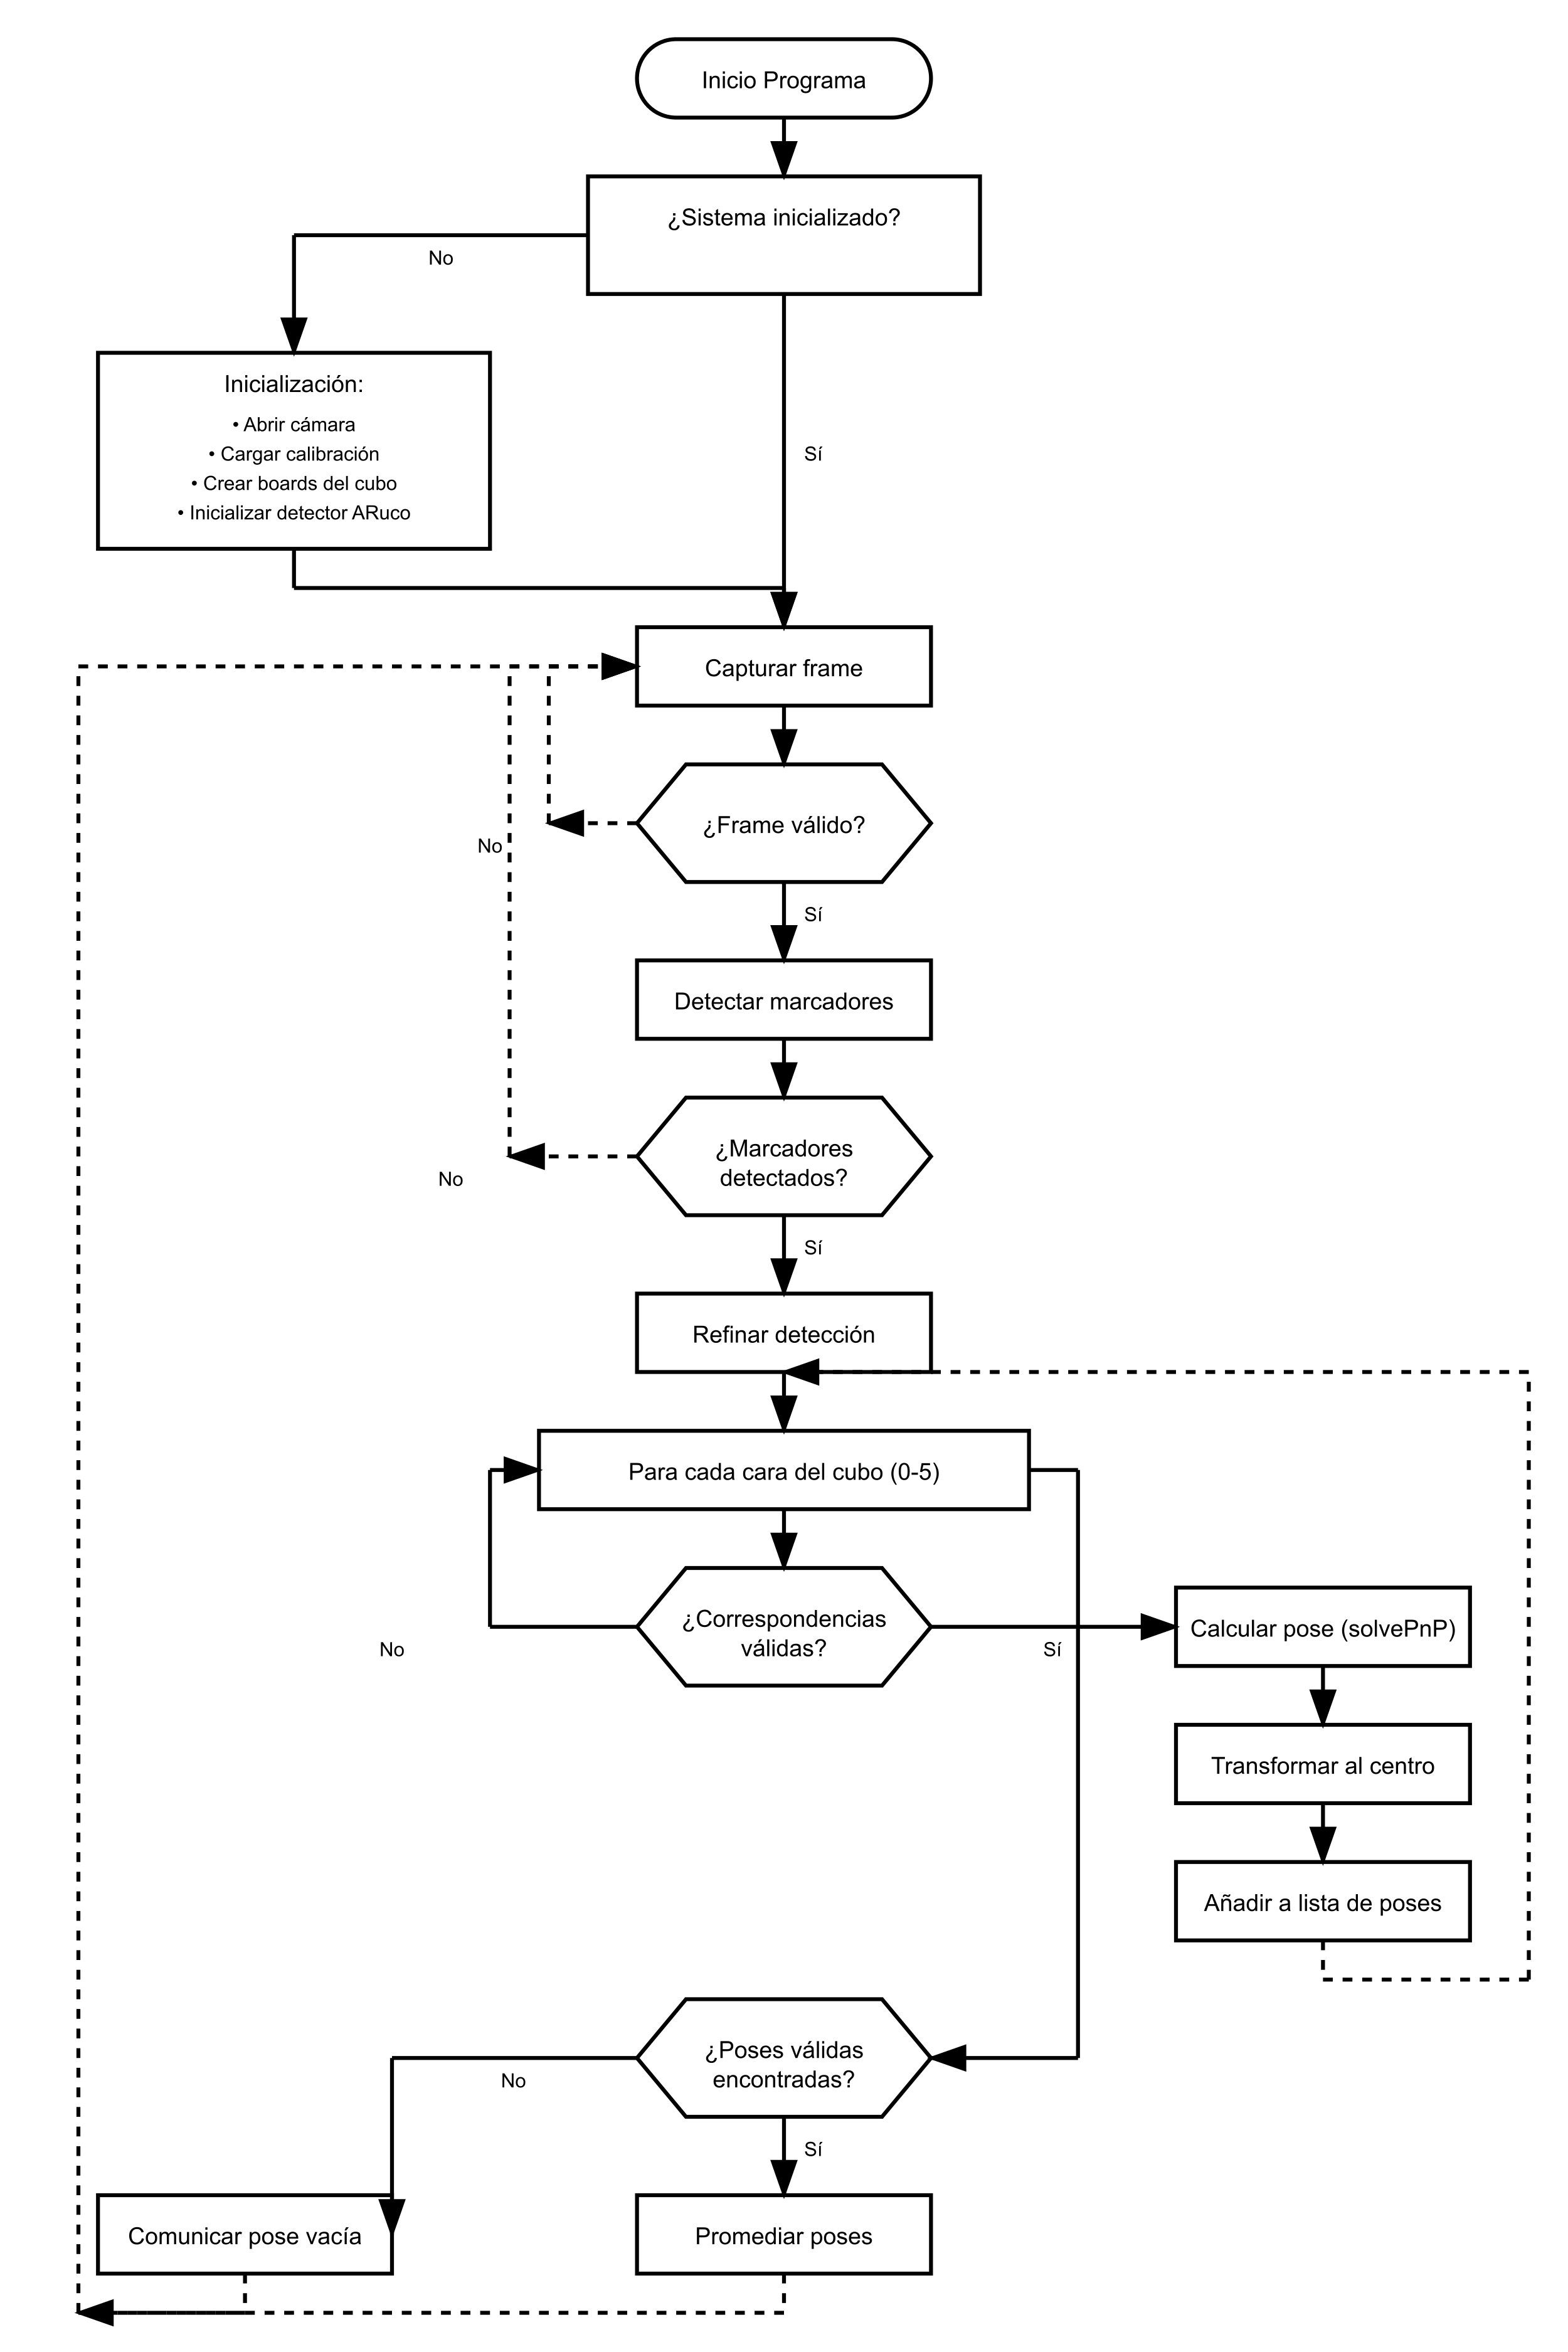
\includegraphics[width=1.0\textwidth]{imaxes/flujo_tfg_correcto.png}
	\caption{Diagrama de flujo detallado del sistema de tracking implementado.}
	\label{fig:flujo_tfg_detallado}
\end{figure}

\section{Planificación temporal detallada}

\begin{figure}[h!]
  \centering
  \begin{ganttchart}[
    hgrid,
    vgrid,
    time slot unit=day,
    x unit=0.5cm,
    y unit chart=0.5cm,
    bar height=0.5,
    bar/.style={fill=udcpink!50},
    group/.style={draw=black, fill=udcgray!25},
    title/.style={draw=none, fill=none},
    title height=1,
    group top shift=0.3,
    group height=0.25,
    bar top shift=0.3,
    title label anchor/.style={below=-1.6ex},
    bar label anchor/.style={left=1ex},
    group label anchor/.style={left=1ex},
    bar label font=\footnotesize,
    group label font=\footnotesize
  ]{1}{20}
    \gantttitle{Planificación Completa del Proyecto (semanas)}{20} \\
    \gantttitlelist{1,...,20}{1} \\
    \ganttgroup{Sprint 1: Extracción TC}{1}{2} \\
    \ganttbar{Importar datos DICOM (T1)}{1}{1} \\
    \ganttbar{Generar secciones (T2)}{1}{2} \\
    \ganttbar{Arreglar modelo (T3)}{2}{2} \\
    \ganttbar{Imprimir modelo (T4)}{2}{2} \\[grid]
    \ganttgroup{Sprint 2: Diseño marcador}{3}{7} \\
    \ganttbar{Instalar librerías (T5)}{3}{3} \\
    \ganttbar{Familiarizar librería (T6)}{3}{4} \\
    \ganttbar{Prototipar pruebas (T7)}{4}{6} \\
    \ganttbar{Implementar tracking (T8)}{5}{7} \\
    \ganttbar{Testear prototipos (T9)}{6}{7} \\
    \ganttbar{Generar modelo final (T10)}{7}{7} \\[grid]
    \ganttgroup{Sprint 3: Integración Exposure}{8}{10} \\
    \ganttbar{Imprimir prototipo (T11)}{8}{9} \\
    \ganttbar{Instalar Exposure (T12)}{8}{10} \\
    \ganttbar{Familiarizar software (T13)}{9}{10} \\[grid]
    \ganttgroup{Sprint 4: Passthrough}{11}{13} \\
    \ganttbar{Implementar captura (T14)}{11}{12} \\
    \ganttbar{Integrar tracking (T15)}{12}{13} \\
    \ganttbar{Validar sistema (T16)}{13}{13} \\[grid]
    \ganttgroup{Sprint 5: Motor independiente}{14}{18} \\
    \ganttbar{Diseñar alternativa (T17)}{14}{15} \\
    \ganttbar{Implementar OpenGL (T18)}{15}{17} \\
    \ganttbar{Validar solución (T19)}{17}{18} \\[grid]
    \ganttgroup{Documentación y cierre}{18}{20} \\
    \ganttbar{Redacción memoria (T20)}{18}{19} \\
    \ganttbar{Revisión final (T21)}{19}{20} \\
  \end{ganttchart}
  \caption{Diagrama de Gantt completo del proyecto mostrando todos los sprints, tareas y dependencias temporales.}
  \label{fig:gantt_completo}
\end{figure}

\section{Tabla detallada de tareas del proyecto}

\begin{table}[h!]
  \centering
  \rowcolors{2}{white}{udcgray!25}
  \begin{tabular}{|c|p{7.5cm}|c|c|}
  \hline
  \rowcolor{udcpink!25}
  \textbf{Nº} & \textbf{Funcionalidad} & \textbf{Est. (H)} & \textbf{Sprint} \\\hline
  1     &   Importar datos en formato DICOM en 3D Slicer    &   2     & 1 \\
  2     &   Generar secciones para poder exportar de 3DSlicer &   40    & 1 \\
  3     &   Arreglar el modelo para que sea viable para impresión &   12    & 1 \\
  4     &   Imprimir modelo                                  &   15    & 1 \\
  5     &   Instalar librerías necesarias para el desarrollo &   4     & 2 \\
  6     &   Familiarizarse con la librería                   &   12    & 2 \\
  7     &   Prototipar pruebas para tests                    &   40    & 2 \\
  8     &   Implementar herramienta para tracking del marcador &   40    & 2 \\  
  9     &   Testear prototipos                               &   25    & 2 \\
  10    &   Generar modelo a partir del prototipo final      &   33    & 2 \\
  11    &   Imprimir prototipo final                         &   16    & 3 \\
  12    &   Instalar y compilar Exposure Render              &   80    & 3 \\
  13    &   Familiarizarse con Exposure Render               &   20    & 3 \\
  14    &   Implementar captura de imagen                    &   30    & 4 \\
  15    &   Integrar sistema de tracking                     &   40    & 4 \\
  16    &   Validar sistema integrado                        &   15    & 4 \\
  17    &   Diseñar motor de render alternativo              &   25    & 5 \\
  18    &   Implementar solución OpenGL                      &   60    & 5 \\
  19    &   Validar solución independiente                   &   20    & 5 \\
  20    &   Redacción de memoria                             &   80    & 6 \\
  21    &   Revisión final del proyecto                      &   15    & 6 \\
  \hline
  \multicolumn{2}{|c|}{\textbf{Total}} & \textbf{584} & \\
  \hline
  \end{tabular}
  \caption{Tabla completa de tareas del proyecto con estimaciones detalladas y asignación a sprints.}
  \label{tab:tareas_completa}
\end{table}
